\chapter{Implementation}
\label{sec:implementation}

\section{Automata}
TODO What we learned when we created the automata and the simple function that we are gonna use for data collection.

\subsection{Sugar Amount}\label{subsec:sugar-amount}
To calibrate the sugar dispensing system, we measured ten times the amount of sugar released over durations of 0.5s, 1s, 1.5s and 2s (2s slightly overflowed the spoon)with each setting tested in multiple trials. The resulting median values were 8.50g, 12.63g, and 16.64g, 20.58g respectively. These findings confirmed a roughly linear relationship between dispensing duration and sugar quantity. For all subsequent trials and modeling efforts, we standardized the input to 1s of sugar dispensing so 12.63g.

\subsection{Waiting Time}
The time the robot arm waits until sugar starts flowing out of the spinner. The cold start time was a variable used for the first time (102s) with an environment of ~25C, our digital twin will leave this variable unneeded. Since it will already know how to act with the actual temperature of the spinner.
At the end of the thesis we will see the variance of this time, based mostly on how warm the spinner will be before.

\subsection{Cooking Time}
The default cooking time is 105s. This starts once the sugar starts flowing out of the spinner. probably becauase the spinner has reached the desired temperature for more than (10-20 seconds). (TODO: Be sure about this)
The spinning time is always 3.75s.
105/3.75 = 28 spins per run.

\subsection{Cooldown Time}
The cooldown time is the time that the spinner runs without the heat, to cool down after the production run. This is needed to avoid burning the sugar in the next run. The default cooldown time is 60s, but we are gonna research how good the quality is gonna be if we increase or decrease this value. 
The Machine manual empfehlen to wait 120s, but we started with 60s bc we noticed a lot room for improvement while using the automata and sometimes it takes a long time to start the next process again to put the sugar and turnon the machien again makes it roughly 120s anyway.

\subsection{Cotton Candy iteration}
We are gonna store which cotton candy iteration we are on, since the last time the machine has been cleaned. We already noticed what a big difference it can make on the quality when the machine has run for a long time without cleaning. 
We want to find the optimal value of iterations we want to run before cleaning the machine. We will start with max 20 iterations.
We will clean the machine and declog the sugar of the spinner with water.


\section{Energy Consumption Measurement}
\label{sec:energy-measurement}

Energy consumption is measured and stored for each production cycle to enable optimization of process parameters for energy efficiency. This measurement, combined with quality metrics, allows the digital twin system to find optimal parameter settings that minimize energy consumption while maintaining product quality.

\subsection{Data Acquisition and Calculation}

Power consumption is measured using a smart plug at 2-second intervals throughout the production process. Total energy consumption is calculated using trapezoidal integration of discrete power measurements:

\[
E = \sum_{i=1}^{n} \frac{P_{i-1} + P_i}{2} \cdot \Delta t_i
\]

where $P_i$ is the power measurement at time $t_i$ and $\Delta t_i$ is the time interval between measurements. The result is converted from Watt-seconds to Watt-hours for practical interpretation of the 5-minute production cycles.

This methodology captures energy consumption across all production phases (startup, heating, spinning, cooldown) and provides the optimization target for energy-efficient cotton candy production.

% \subsection{Power Data Acquisition}
% 
% Power consumption data is collected using a smart plug (Tasmota-compatible device) that measures electrical parameters at 2-second intervals throughout the production process. The plug captures instantaneous power values in Watts, which are logged with precise timestamps in the process execution system (XES) format. Given the short duration of cotton candy production (maximum 5 minutes), this sampling frequency provides sufficient temporal resolution for accurate energy integration.
% 
% \subsection{Energy Calculation Methodology}
% 
% Total energy consumption for each production cycle is calculated using trapezoidal numerical integration of the discrete power measurements over time. This approach accounts for the varying power draw during different phases of the cotton candy making process (heating, spinning, cooling).
% 
% The energy calculation follows the fundamental relationship:
% \[
% E = \int_{t_0}^{t_f} P(t) \, dt
% \]
% 
% where $E$ is the total energy consumed, $P(t)$ is the instantaneous power at time $t$, $t_0$ is the process start time, and $t_f$ is the process end time.
% 
% For discrete measurements taken at intervals $\Delta t = 2$ seconds, the trapezoidal rule approximates this integral as:
% 
% \[
% E \approx \sum_{i=1}^{n} \frac{P_{i-1} + P_i}{2} \cdot \Delta t_i
% \]
% 
% where:
% \begin{itemize}
%     \item $P_i$ is the power measurement at time $t_i$
%     \item $\Delta t_i = t_i - t_{i-1}$ is the time interval between consecutive measurements
%     \item $n$ is the total number of measurement intervals
% \end{itemize}
% 
% The result is expressed in Watt-seconds (Joules), which is then converted to Watt-hours by dividing by 3600:
% 
% \[
% E_{Wh} = \frac{E_{Ws}}{3600}
% \]
% 
% For the typical 5-minute cotton candy production process, Watt-hours provide a more intuitive unit than kilowatt-hours, which would result in very small decimal values.
% 
% \subsection{Process Phase Integration}
% 
% The energy calculation spans the complete production cycle, from process initiation to final cooldown. Key phases include:
% 
% \begin{enumerate}
%     \item \textbf{Startup phase}: Initial power draw as the spinner begins heating
%     \item \textbf{Heating phase}: High power consumption to reach operating temperature
%     \item \textbf{Production phase}: Active spinning and sugar melting with varying power draw
%     \item \textbf{Cooldown phase}: Reduced power consumption during cooling period
% \end{enumerate}
% 
% By integrating power consumption across all phases, the methodology captures the total energy cost of each cotton candy unit, enabling optimization of process parameters for energy efficiency while maintaining product quality.
% 
% \subsection{Data Quality Considerations}
% 
% The trapezoidal integration method assumes linear interpolation between discrete measurement points. While this introduces some approximation error, the 2-second sampling interval is sufficiently fine-grained relative to the thermal and mechanical time constants of the cotton candy machine to provide accurate energy estimates. Additionally, the method handles variable time intervals between measurements, accommodating any minor variations in data logging frequency.


\section{Product Quality Measurement}
% Stichpunkte:
% - During each run, collect product-related measurements
% - Store data in structured dataset
% - Used to evaluate output quality
% - Includes input sugar, output weight, volume, etc.

During the data collection phase, a structured dataset was compiled by recording relevant product-related parameters during each cotton candy production run. These measurements include the input sugar weight, the final cotton candy weight, estimated volume based on geometry, and the derived Fluffiness Index. This enabled consistent tracking across experiments and formed the basis for downstream quality evaluation and performance comparisons for the Model.

\subsection{Weight Measurement}

% Stichpunkte:
% - Manually weigh sugar before each run (input)
% - Weigh finished cotton candy on stick
% - Subtract known stick weight to get net cotton candy weight
% - Use same digital scale throughout
% - Needed for yield and fluffiness index

The input mass of sugar for each production run was manually measured using a precision scale with a readability of 0.01 grams. To determine the output mass of the produced cotton candy, the final product (including the stick) was weighed immediately after production using the same scale. The net weight of the cotton candy was then computed by subtracting the known weight of the stick, which was measured prior to the experiment and kept constant across all runs.

Accurate weight measurement was essential for evaluating the amount of produced cotton candy and for computing derived metrics such as the quality and Fluffiness Index. All weights were recorded in grams with a precision of two decimal places.



% TODO: Change Image to a better and smaller one, this is just a placeholder
% \begin{figure}[H]
%         \caption{Comparison between geometric approximation and real cotton candy morphology}
%     \label{fig:volume-comparison}
%     \centering
%         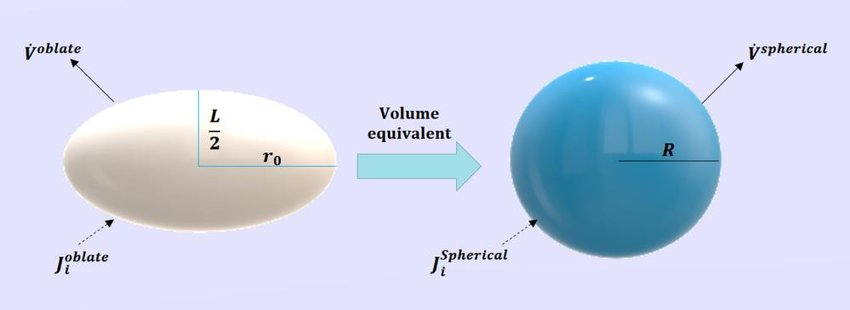
\includegraphics[width=\textwidth]{figures/Schematic-diagram-of-the-oblate-spheroid-and-its-volume-equivalent-sphere.jpg}
%         % \caption{Idealized oblate spheroid}
%         \label{fig:oblate-spheroid}
% \end{figure}
% \begin{figure}[H]
%         \centering
%         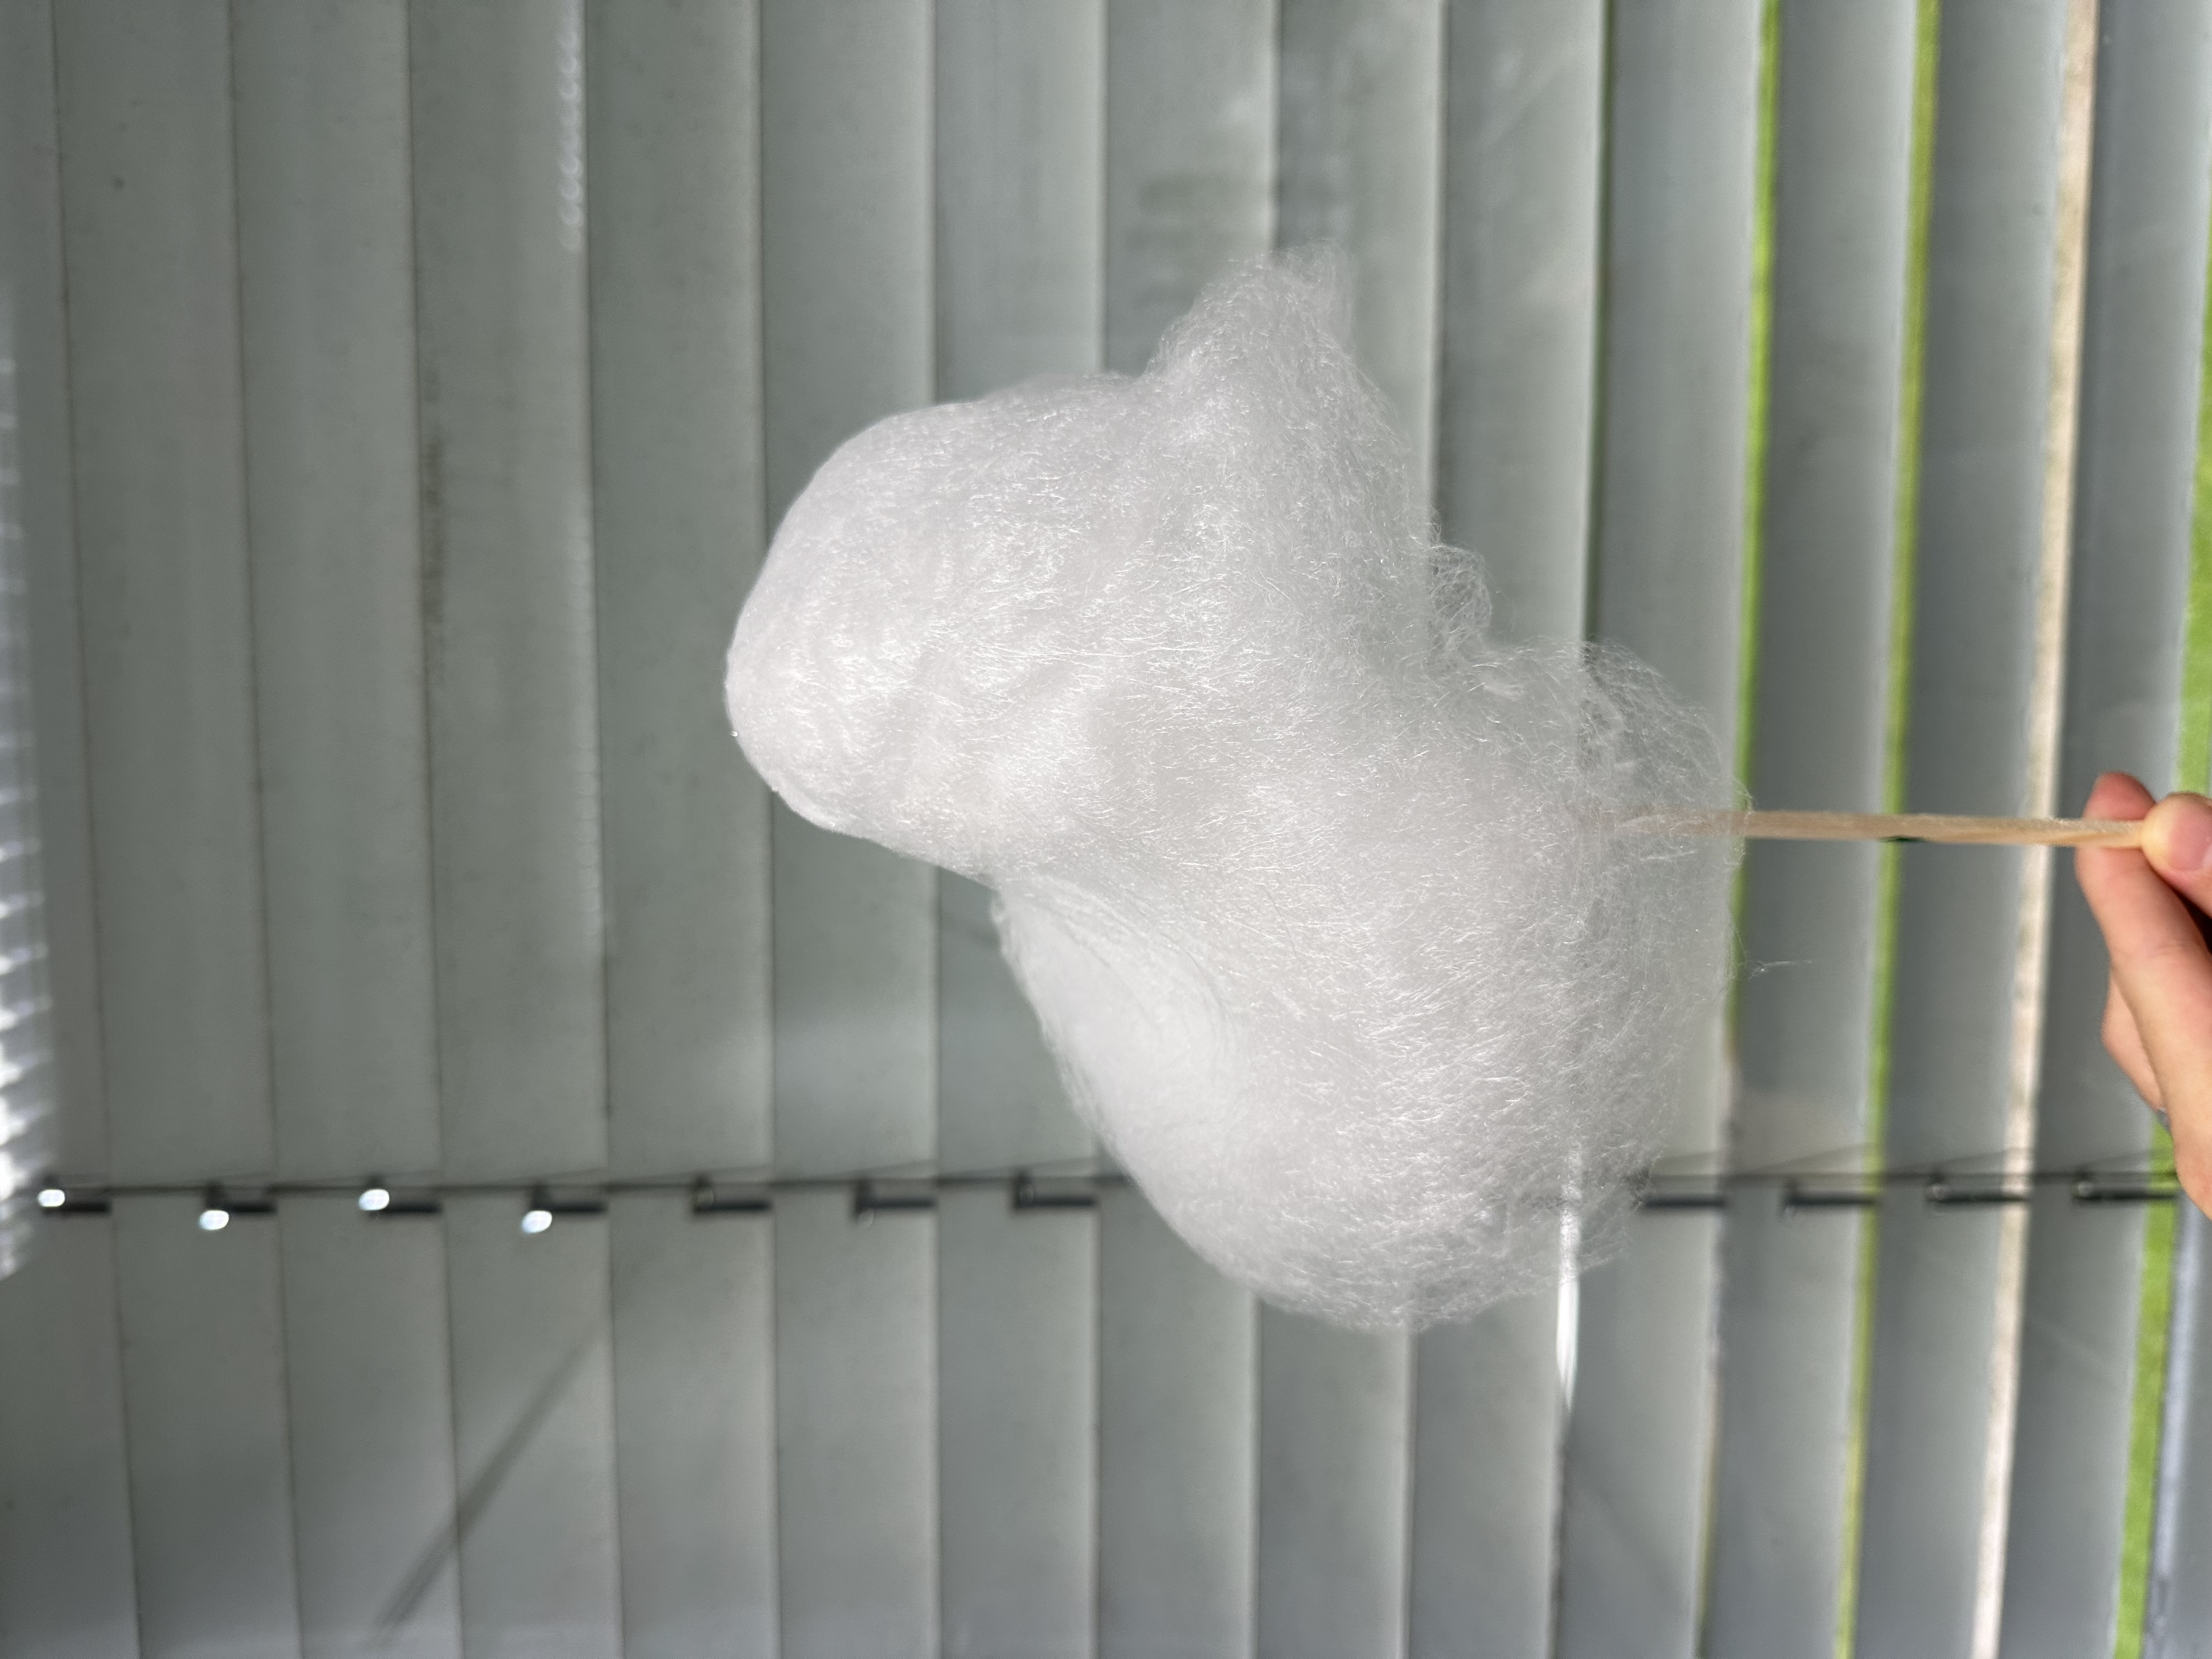
\includegraphics[width=\textwidth]{figures/firstCC.jpeg}
%         \caption{Actual cotton candy output}
%         \label{fig:cotton-candy}
% \end{figure}

\subsection{Volume Estimation}
% Stichpunkte:
% - You describe in detail how you estimate volume.
% - You assume the shape is an oblate spheroid (like a UFO).
% - You measure height and width with a ruler.
% - You apply the formula V = 4/3 * pi * a^2 * c
% - You derive a Fluffiness Index = Volume / Weight.

To approximate the spatial characteristics of the cotton candy output, the product was modeled as an oblate spheroid — a flattened ellipsoid shape that approximates the typical morphology observed during production.

\begin{figure}[H]
    \centering
    \begin{subfigure}[b]{0.45\textwidth}
        \centering
        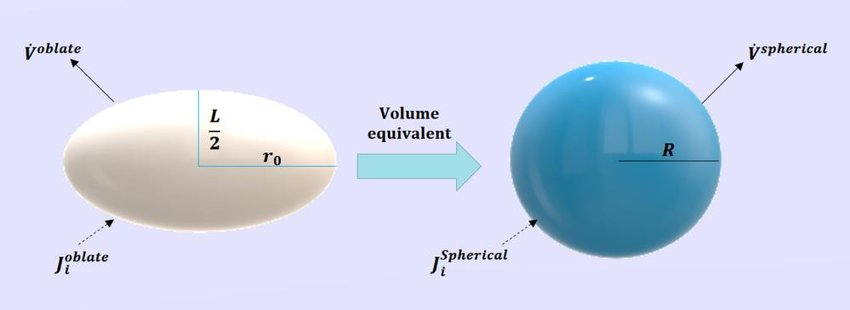
\includegraphics[width=\textwidth]{figures/Schematic-diagram-of-the-oblate-spheroid-and-its-volume-equivalent-sphere.jpg}
        \caption{Idealized oblate spheroid}
        \label{fig:oblate-spheroid}
    \end{subfigure}
    \hfill
    \begin{subfigure}[b]{0.45\textwidth}
        \centering
        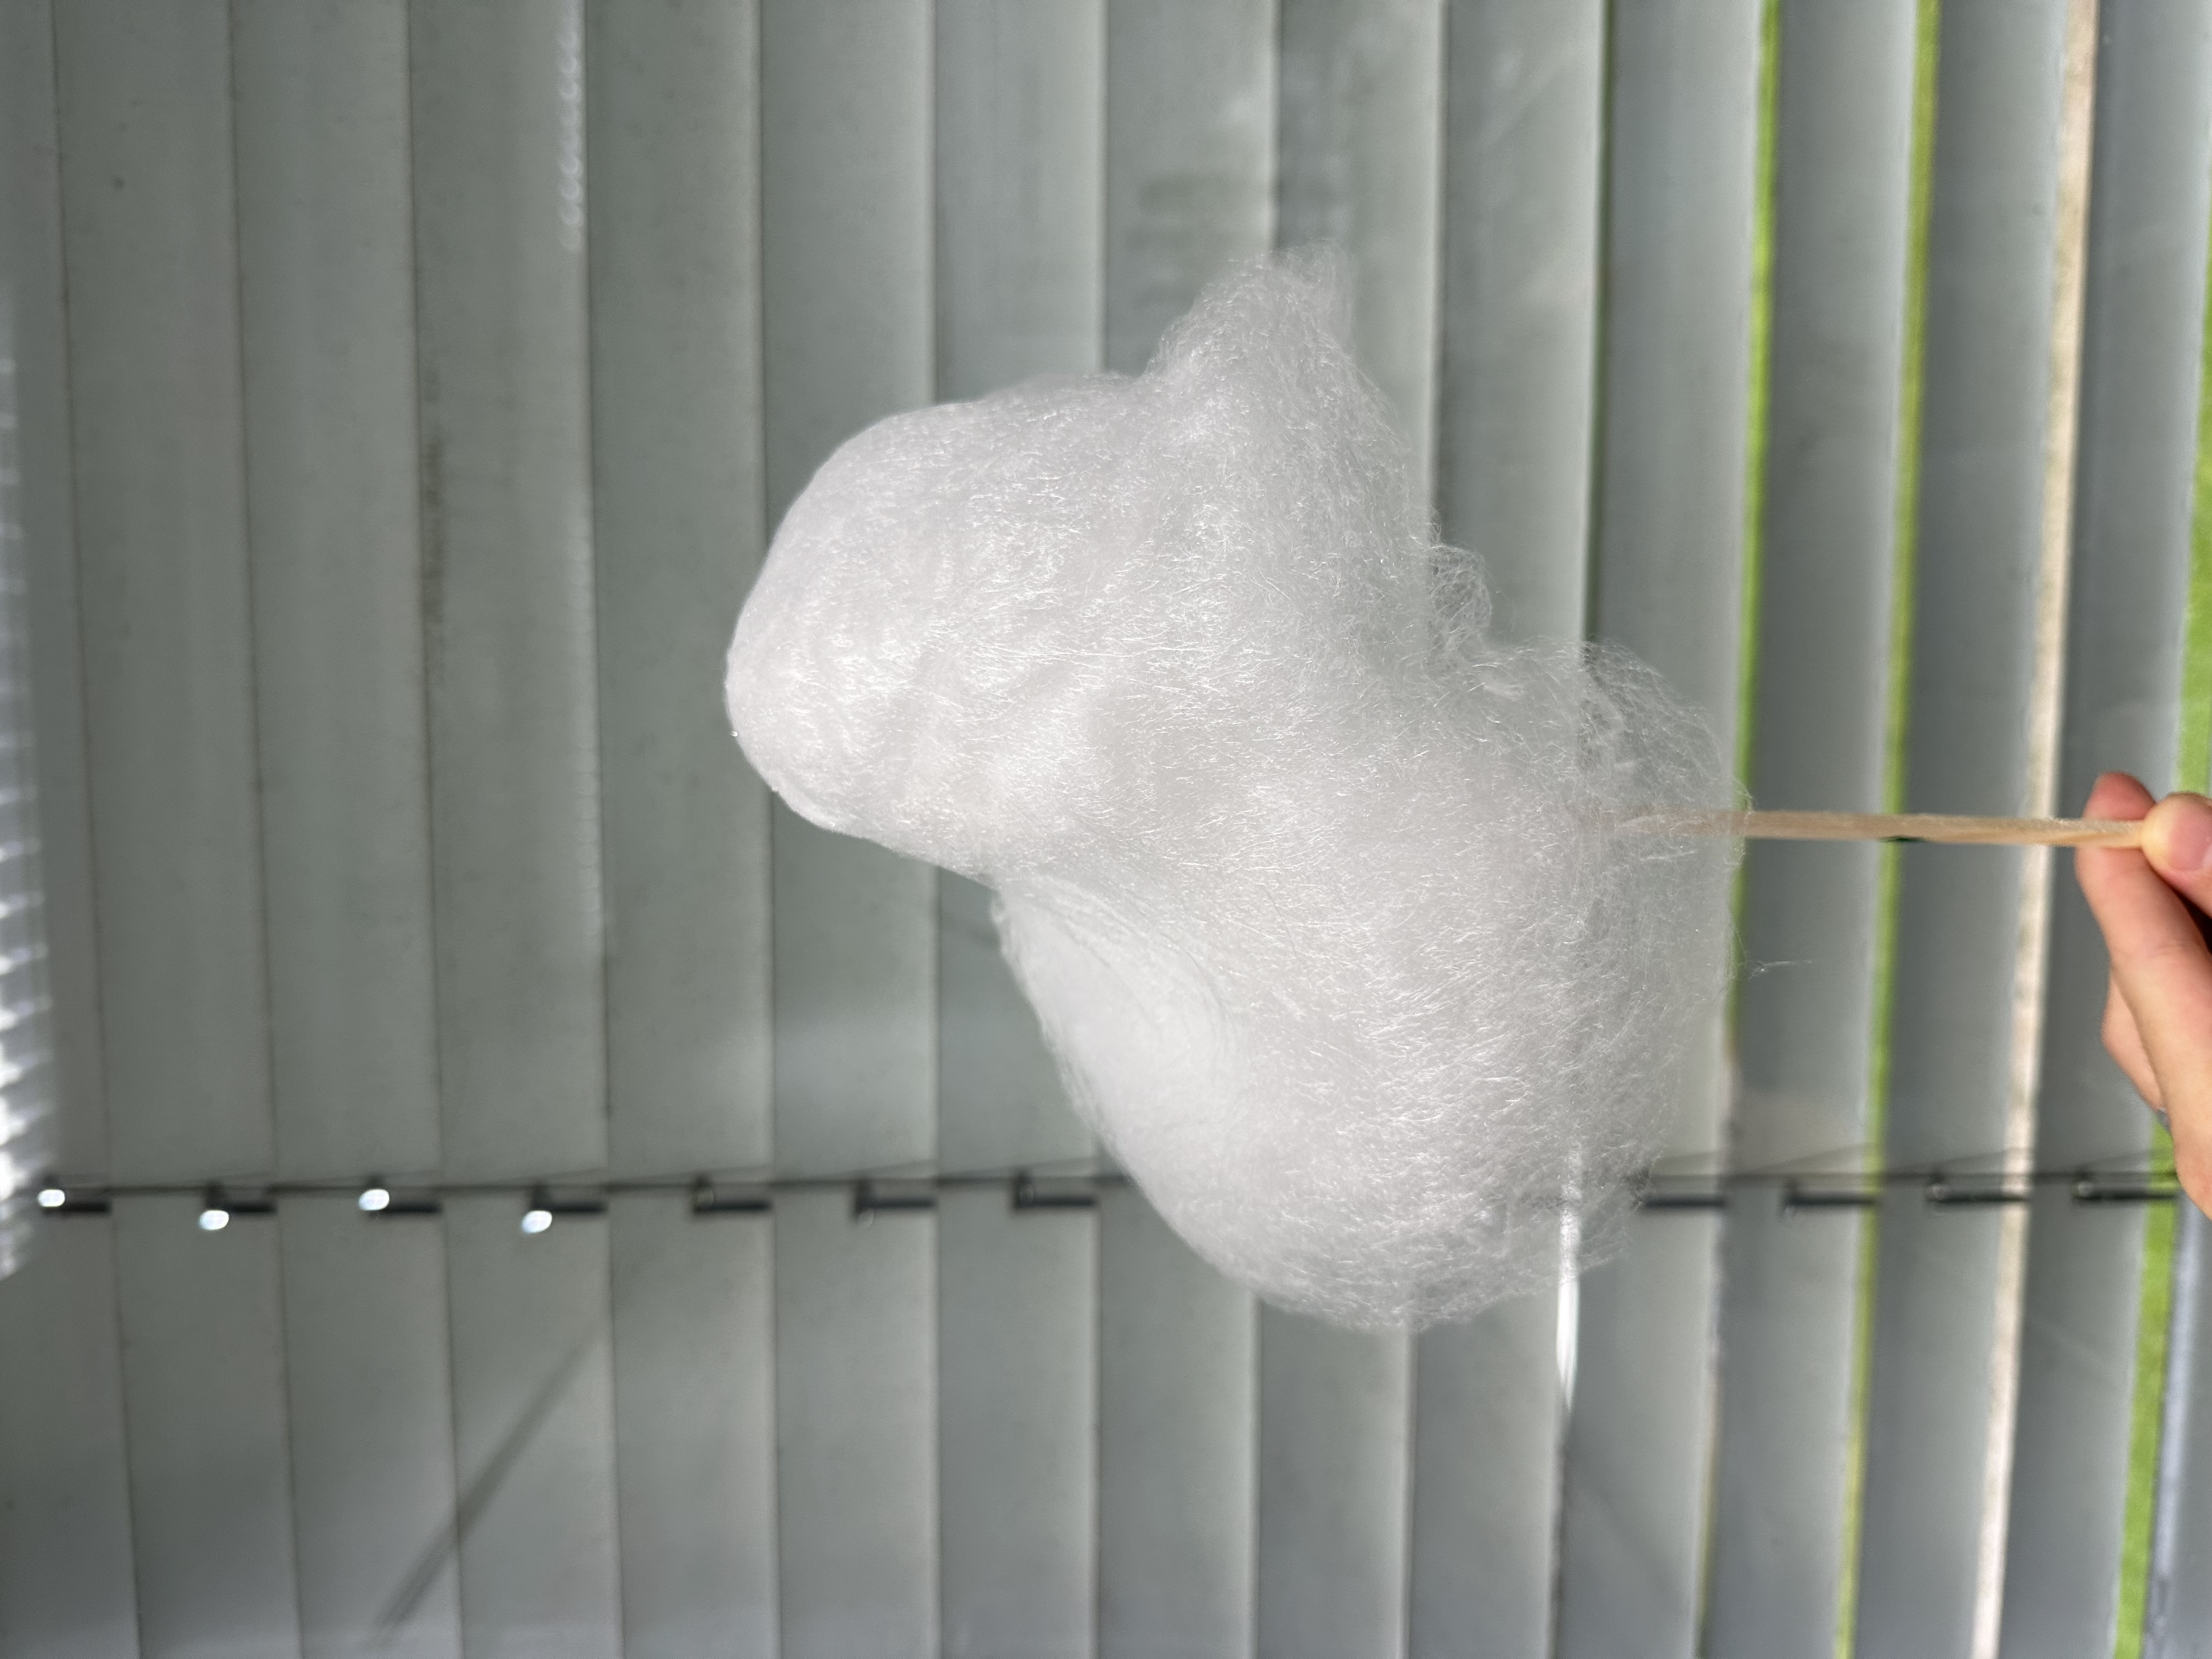
\includegraphics[width=\textwidth]{figures/firstCC.jpeg}
        \caption{Actual cotton candy output}
        \label{fig:cotton-candy}
    \end{subfigure}
    \caption{Comparison between geometric approximation and real cotton candy morphology}
    \label{fig:volume-comparison}
\end{figure}

Measurements of the maximum width and height were taken manually using a standard ruler immediately after each production run. Based on these dimensions, the volume \( V \) was estimated using the standard formula for an oblate spheroid:

\[
V = \frac{4}{3} \pi a^2 c
\]

where \( a \) is the equatorial radius (half of the width) and \( c \) is the polar radius (half of the height). Although this approach does not capture fine-grained structural variations, it offers a practical and repeatable method to compare volumetric differences across runs.

To further assess structural quality, a Fluffiness Index was derived as:

\[
\text{Fluffiness Index} = \frac{V}{\text{Weight}}
\]

This index serves as a proxy for the density of the cotton candy, with higher values indicating a lighter, airier structure. The same procedure and tools were applied consistently across all production runs to ensure internal comparability.

\subsection{Limitations in Volume Measurement}

The estimation of cotton candy volume relied on manual measurements of width and height, followed by geometric approximation. While this method provides a reasonable basis for comparative analysis, it is subject to several limitations: (a) the inherently irregular and fragile structure of cotton candy, (b) potential observer bias during manual measurement, and (c) the assumption of a regular geometric shape. As such, the absolute values of estimated volume should be interpreted with caution. However, because the same procedure was applied uniformly across all experimental runs, the relative differences and trends derived from this method remain valid for assessing the effects of the digital twin optimization.

\section{Feature Engineering for Decision Tree Optimization}
\label{sec:feature-engineering}

To enable effective machine learning optimization, the raw process data was transformed into a structured feature vector suitable for decision tree modeling. This preprocessing involved careful selection and organization of variables to maximize predictive power while minimizing redundancy and computational complexity.

\subsection{Feature Vector Structure}

The final feature vector consists of 28 carefully selected features organized in a logical hierarchy:

\begin{enumerate}
    \item \textbf{Process Parameters (6 features):} Core decision variables including iteration since maintenance, wait time, cook time, cooldown time, and derived timing metrics (duration until handover and total duration)
    \item \textbf{Environmental Baseline (2 features):} External humidity and temperature captured at process initiation to establish ambient conditions
    \item \textbf{Internal Environmental Dynamics (20 features):} Four internal sensors measured across five critical process phases:
    \begin{itemize}
        \item Internal humidity (InH) and temperature (InT) sensors
        \item Infrared ambient temperature (IrA) at the sensor location
        %\item Infrared object temperature (IrO) of the rotating cotton candy machine head, which correlates with the actual internal head temperature (e.g., IrO = 81.55 corresponds to actual internal temperature ≈ 178°C, like we saw before)
    \end{itemize}
\end{enumerate}

\subsection{Redundancy Elimination Strategy}


Analysis of environmental sensor data revealed significant redundancy in external measurements, where external humidity and temperature remained virtually constant throughout the production process (±0.4\% and ±0.1°C variation respectively). To optimize the feature set:

\begin{itemize}
    \item \textbf{External sensors} were reduced from 10 measurements (2 sensors × 5 phases) to 2 baseline measurements, capturing ambient conditions without repetitive data
    \item \textbf{Internal sensors} were retained across all 5 phases, as they exhibited substantial variation (internal humidity: -27\% change, internal temperature: +15°C change, infrared ambient temperature and machine head object temperature: up to +58 units variation)
\end{itemize}

This optimization reduced the environmental feature space from 30 to 22 features while preserving all meaningful environmental dynamics, resulting in a 22\% reduction in feature dimensionality without information loss.

\subsection{Process Phase Identification}

Five critical process phases were identified for environmental monitoring:

\begin{enumerate}
    \item \textbf{Before turn-on:} Baseline internal conditions prior to machine activation
    \item \textbf{After flow start:} Environmental state during active cotton candy production
    \item \textbf{After flow end:} Conditions immediately following production completion
    \item \textbf{After weigh start:} Environmental state at cooling phase initiation
    \item \textbf{End:} Final environmental conditions post-cooling
\end{enumerate}

This temporal sampling strategy captures the complete thermal and humidity evolution during cotton candy production, enabling the decision tree to learn correlations between environmental conditions and process outcomes.
